\documentclass{article}
\usepackage[utf8]{inputenc}
\usepackage{tikz}
\usetikzlibrary{shapes.geometric, arrows}

\tikzstyle{data} = [circle, draw=black, fill=red!30]
\tikzstyle{arrow} = [-stealth]

\begin{document}

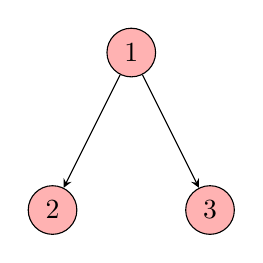
\begin{tikzpicture}[node distance = 2cm]
    \node (a) [data] {1};
    \node (b) [data, below of=a, xshift=-1cm] {2};
    \node (c) [data, below of=a, xshift=1cm] {3};

    \draw[arrow] (a) -- (b);
    \draw[arrow] (a) -- (c);
\end{tikzpicture}

\end{document}
